\documentclass[8pt,a4paper,compress]{beamer}

\usepackage{/home/siyer/lib/slides}

\title{Basic Data Structures}
\date{}

\begin{document}
\begin{frame}
\vfill
\titlepage
\end{frame}

\begin{frame}
\frametitle{Outline}
\tableofcontents
\end{frame}

\section{Some Java Preliminaries}
\begin{frame}[fragile]
\begin{itemize}
\item generics (aka parametrized types) is a Java mechanism that enables the implementation of collection ADTs that can be used to store any type of data

\begin{lstlisting}[language=Java]
Stack<String> stack = new Stack<String>();
stack.push("Test");
...
String next = stack.pop();
\end{lstlisting}

\begin{lstlisting}[language=Java]
Queue<Date> queue = new Queue<Date)();
queue.enqueue(new Date(3, 14, 1879));
...
Date next = queue.dequeue();
\end{lstlisting}

\item type parameters have to be instantiated as reference types, so Java allows generic code to be used with primitive types by automatically converting (auto boxing) them to their corresponding (wrapper) reference types and vice versa (auto unboxing)
\begin{lstlisting}[language=Java]
Stack<Integer> stack = new Stack<Integer>();
stack.push(42);      // auto boxing (int -> Integer)
int i = stack.pop(); // auto unboxing (Integer -> int)
\end{lstlisting}

\item iterable collections can be enumerated using foreach statement 
\begin{lstlisting}[language=Java]
Bag<Integer> numbers = new Bag<Integer>();
...
for (int x : numbers) { StdOut.println(x); }
\end{lstlisting}

which translates to 

\begin{lstlisting}[language=Java]
Iterator<Integer> iter = numbers.iterator();
while (iter.hasNext()) { StdOut.println(iter.next()); }
\end{lstlisting}
\end{itemize}
\end{frame}

\section{Linked Lists}
\begin{frame}[fragile]
\begin{itemize}
\item a linked list is a recursive data structure that is either empty (\lstinline{null}) or a reference to a node having a generic item and a reference to a linked list

\item node record 
\begin{lstlisting}[language=Java]
private class Node {
    Item item; // generic item
    Node next;
}
\end{lstlisting}

\item traversal
\begin{lstlisting}[language=Java]
for (Node x = first; x != null; x = x.next) {

    // do something with x.item.
    
}
\end{lstlisting}
\end{itemize}
\end{frame}

\begin{frame}[fragile]
\begin{itemize}
\item building a linked list
\begin{lstlisting}[language=Java]
Node first = new Node();
first.item = "to";
\end{lstlisting}

\begin{center}
\includegraphics[scale=0.7]{{./figures/llist1.1}.pdf}
\end{center}

\begin{lstlisting}[language=Java]
Node second = new Node();
second.item = "be";
first.next = second;
\end{lstlisting}

\begin{center}
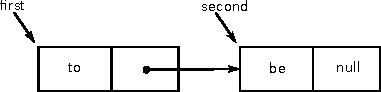
\includegraphics[scale=0.7]{{./figures/llist1.2}.pdf}
\end{center}

\begin{lstlisting}[language=Java]
Node third = new Node();
third.item = "or";
second.next = third;
\end{lstlisting}

\begin{center}
\includegraphics[scale=0.7]{{./figures/llist1.3}.pdf}
\end{center}
\end{itemize}
\end{frame}

\begin{frame}[fragile]
\begin{itemize}
\item insert at the beginning
\begin{lstlisting}[language=Java]
Node oldfirst = first;
\end{lstlisting}

\begin{center}
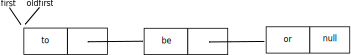
\includegraphics[scale=0.7]{{./figures/llist2.1}.pdf}
\end{center}

\begin{lstlisting}[language=Java]
first = new Node();
first.item = "not";
\end{lstlisting}

\begin{center}
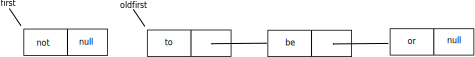
\includegraphics[scale=0.7]{{./figures/llist2.2}.pdf}
\end{center}

\begin{lstlisting}[language=Java]
first.next = oldfirst;
\end{lstlisting}

\begin{center}
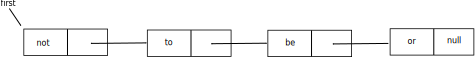
\includegraphics[scale=0.7]{{./figures/llist2.3}.pdf}
\end{center}
\end{itemize}
\end{frame}

\begin{frame}[fragile]
\begin{itemize}
\item remove from the beginning
\begin{lstlisting}[language=Java]
first = first.next;
\end{lstlisting}

\begin{center}
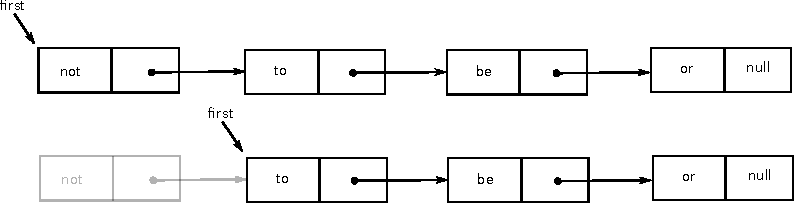
\includegraphics[scale=0.7]{./figures/llist3.pdf}
\end{center}
\end{itemize}
\end{frame}

\begin{frame}[fragile]
\begin{itemize}
\item insert at the end
\begin{lstlisting}[language=Java]
Node oldlast = last;
\end{lstlisting}

\begin{center}
\includegraphics[scale=0.7]{{./figures/llist4.1}.pdf}
\end{center}

\begin{lstlisting}[language=Java]
last = new Node();
last.item = "not";
\end{lstlisting}

\begin{center}
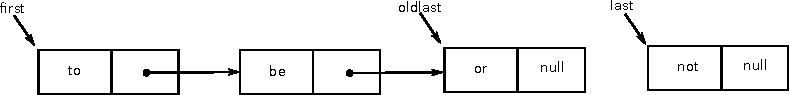
\includegraphics[scale=0.7]{{./figures/llist4.2}.pdf}
\end{center}

\begin{lstlisting}[language=Java]
oldlast.next = last;
\end{lstlisting}

\begin{center}
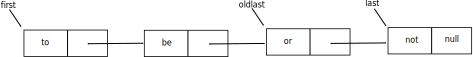
\includegraphics[scale=0.7]{{./figures/llist4.3}.pdf}
\end{center}
\end{itemize}
\end{frame}

\section{Bags}
\begin{frame}[fragile]
\begin{itemize}
\item a bag is an iterable collection that provides clients with the ability to collect items

\item \lstinline{Bag} API
\begin{lstlisting}[language={}]
public interface Bag<Item> extends Iterable<Item> 

    boolean isEmpty()   // is the bag empty?
    int size()          // number of items in the bag
    void add(Item item) // add an item
\end{lstlisting}

\item \lstinline{Bag} client
\begin{lstlisting}[language=Java]
public class Stats {
    public static void main(String[] args) {
        LinkedBag<Double> numbers = new LinkedBag<Double>();
        while (!StdIn.isEmpty()) { numbers.add(StdIn.readDouble()); }
        int N = numbers.size();
        double sum = 0.0;
        for (double x : numbers) { sum += x; }
        double mean = sum / N;
        sum = 0.0;
        for (double x : numbers) { sum += (x - mean) * (x - mean); }
        double std = Math.sqrt(sum / (N - 1));
        StdOut.printf("Mean:    %.2f\n", mean);
        StdOut.printf("Std dev: %.2f\n", std);
    }
}
\end{lstlisting}

\begin{lstlisting}[language={}]
$ java Stats
100 99 101 120 98 107 109 81 101 90
<ctrl-d>
Mean:    100.60
Std dev: 10.51
\end{lstlisting}
\end{itemize}
\end{frame}

\begin{frame}[fragile]
\begin{itemize}
\item \lstinline{Bag} implementation using a linked list
\begin{lstlisting}[language=Java]
import java.util.Iterator;
import java.util.NoSuchElementException;

public class LinkedBag<Item> implements Bag<Item> {
    private int N; 
    private Node<Item> first; 

    private static class Node<Item> {
        private Item item;
        private Node<Item> next;
    }

    public LinkedBag() {
        first = null;
        N = 0;
    }

    public boolean isEmpty() { return first == null; }

    public int size() { return N; }

    public void add(Item item) {
        Node<Item> oldfirst = first;
        first = new Node<Item>();
        first.item = item;
        first.next = oldfirst;
        N++;
    }
    ...
\end{lstlisting}
\end{itemize}
\end{frame}

\begin{frame}[fragile]
\begin{itemize}
\item \lstinline{Bag} implementation using a linked list (contd.)
\begin{lstlisting}[language=Java]
    ...
    public Iterator<Item> iterator() { 
        return new ListIterator<Item>(first); 
    }

    private class ListIterator<Item> implements Iterator<Item> {
        private Node<Item> current;

        public ListIterator(Node<Item> first) { current = first; }

        public boolean hasNext() { return current != null; }

        public Item next() {
            if (!hasNext()) { throw new NoSuchElementException(); }
            Item item = current.item;
            current = current.next; 
            return item;
        }
        ...
    }
    ...
}
\end{lstlisting}
\end{itemize}
\end{frame}

\section{Queues}
\begin{frame}[fragile]
\begin{itemize}
\item a queue is an iterable collection that is based on the first-in-first-out (FIFO) policy

\item \lstinline{Queue} API
\begin{lstlisting}[language={}]
public interface Queue<Item> extends Iterable<Item>

    boolean isEmpty()       // is the queue empty?
    int size()              // number of items in the queue
    void enqueue(Item item) // add an item
    Item dequeue()          // remove the least recently added item
\end{lstlisting}

\item \lstinline{Queue} client
\begin{lstlisting}[language=Java]
public class ReadInts {
    public static void main(String[] args) {
        LinkedQueue<Integer> q = new LinkedQueue<Integer>();
        while (!StdIn.isEmpty()) { q.enqueue(StdIn.readInt()); }
        for (int i : q) { StdOut.println(i); }
    }
}
\end{lstlisting}

\begin{lstlisting}[language={}]
$ java ReadInts
100 99 101 120 98 107 109 81 101 90
<ctrl-d>
100
99
101
120
98
107
109
81
101
90
\end{lstlisting}
\end{itemize}
\end{frame}

\begin{frame}[fragile]
\begin{itemize}
\item \lstinline{Queue} implementation using a linked list
\begin{lstlisting}[language=Java]
import java.util.Iterator;
import java.util.NoSuchElementException;

public class LinkedQueue<Item> implements Queue<Item> {
    private int N; 
    private Node<Item> first; 
    private Node<Item> last; 

    public LinkedQueue() {
        first = null;
        last  = null;
        N = 0;
    }

    public boolean isEmpty() { return first == null; }

    public int size() { return N; }

    public void enqueue(Item item) {
        Node<Item> oldlast = last;
        last = new Node<Item>();
        last.item = item;
        last.next = null;
        if (isEmpty()) { first = last; }
        else           { oldlast.next = last; }
        N++;
    }
    ...
\end{lstlisting}
\end{itemize}
\end{frame}

\begin{frame}[fragile]
\begin{itemize}
\item \lstinline{Queue} implementation using a linked list (contd.)
\begin{lstlisting}[language=Java]
    ...
    public Item dequeue() {
        if (isEmpty()) { 
            throw new NoSuchElementException("Queue underflow"); 
        }
        Item item = first.item;
        first = first.next;
        N--;
        if (isEmpty()) { last = null; }
        return item;
    }

    public Iterator<Item> iterator() { 
        return new ListIterator<Item>(first); 
    }

    private class ListIterator<Item> implements Iterator<Item> {
        private Node<Item> current;

        public ListIterator(Node<Item> first) { current = first; }

        public boolean hasNext() { return current != null; }

        public Item next() {
            if (!hasNext()) { throw new NoSuchElementException(); }
            Item item = current.item;
            current = current.next; 
            return item;
        }
        ...
    }
    ...
}
\end{lstlisting}
\end{itemize}
\end{frame}

\section{Stacks}
\begin{frame}[fragile]
\begin{itemize}
\item a pushdown stack is an iterable collection that is based on the last-in-first-out (LIFO) policy

\item \lstinline{Stack} API
\begin{lstlisting}[language={}]
public interface Stack<Item> extends Iterable<Item>

    boolean isEmpty()    // is the stack empty?
    int size()           // number of items in the stack
    void push(Item item) // add an item
    Item peek()          // most recently added item
    Item pop()           // remove the most recently added item
\end{lstlisting}

\item \lstinline{Stack} client
\begin{lstlisting}[language=Java]
public class Reverse {
    public static void main(String[] args) {
        LinkedStack<Integer> stack = new LinkedStack<Integer>();
        while (!StdIn.isEmpty()) {
            stack.push(StdIn.readInt());
        }
        for (int i : stack) {
            StdOut.println(i);
        }
    }
}
\end{lstlisting}

\begin{lstlisting}[language={}]
$ java Reverse 
1 2 3 4 5
<ctrl-d>
5
4
3
2
1
\end{lstlisting}
\end{itemize}
\end{frame}

\begin{frame}[fragile]
\begin{itemize}
\item \lstinline{Stack} client (Dijkstra's two-stack algorithm for expression evaluation)
\begin{lstlisting}[language=Java]
public class Evaluate {
    public static void main(String[] args) { 
        LinkedStack<String> ops  = new LinkedStack<String>();
        LinkedStack<Double> vals = new LinkedStack<Double>();
        while (!StdIn.isEmpty()) {
            String s = StdIn.readString();
            if      (s.equals("("))    { ; }
            else if (s.equals("+"))    { ops.push(s); }
            else if (s.equals("-"))    { ops.push(s); }
            else if (s.equals("*"))    { ops.push(s); }
            else if (s.equals("/"))    { ops.push(s); }
            else if (s.equals("sqrt")) { ops.push(s); }
            else if (s.equals(")")) {
                String op = ops.pop();
                double v = vals.pop();
                if      (op.equals("+"))    { v = vals.pop() + v; }
                else if (op.equals("-"))    { v = vals.pop() - v; } 
                else if (op.equals("*"))    { v = vals.pop() * v; }
                else if (op.equals("/"))    { v = vals.pop() / v; }
                else if (op.equals("sqrt")) { v = Math.sqrt(v); }
                vals.push(v);
            }
            else vals.push(Double.parseDouble(s));
        }
        StdOut.println(vals.pop());
    }
}
\end{lstlisting}

\begin{lstlisting}[language={}]
$ java Evaluate
( 1 + ( ( 2 + 3 ) * ( 4 * 5 ) ) )
101.0
$ java Evaluate
( ( 1 + sqrt ( 5.0 ) ) / 2.0 )
1.618033988749895
\end{lstlisting}
\end{itemize}
\end{frame}

\begin{frame}[fragile]
\begin{itemize}
\item \lstinline{Stack} implementation using a resizing array
\begin{lstlisting}[language=Java]
import java.util.Iterator;
import java.util.NoSuchElementException;

public class ResizingArrayStack<Item> implements Stack<Item> {
    private Item[] a; 
    private int N; 

    public ResizingArrayStack() { a = (Item[]) new Object[2]; }

    public boolean isEmpty() { return N == 0; }

    public int size() { return N; }

    private void resize(int capacity) {
        Item[] temp = (Item[]) new Object[capacity];
        for (int i = 0; i < N; i++) {
            temp[i] = a[i];
        }
        a = temp;
    }

    public void push(Item item) {
        if (N == a.length) { resize(2 * a.length) }; 
        a[N++] = item; 
    }

    public Item peek() {
        if (isEmpty()) {
            throw new NoSuchElementException("Stack underflow");
        }
        return a[N - 1];
    }    
    ...
\end{lstlisting}
\end{itemize}
\end{frame}

\begin{frame}[fragile]
\begin{itemize}
\item \lstinline{Stack} implementation using a resizing array (contd.)
\begin{lstlisting}[language=Java]
    ...    
    public Item pop() {
        if (isEmpty()) { 
            throw new NoSuchElementException("Stack underflow"); 
        }
        Item item = a[N - 1];
        a[N - 1] = null; 
        N--;
        if (N > 0 && N == a.length / 4) { resize(a.length / 2); }
        return item;
    }

    public Iterator<Item> iterator() { return new ReverseArrayIterator(); }

    private class ReverseArrayIterator implements Iterator<Item> {
        private int i;

        public ReverseArrayIterator() { i = N; }

        public boolean hasNext() { return i > 0; }

        public Item next() {
            if (!hasNext()) { throw new NoSuchElementException(); }
            return a[--i];
        }
        ...
    }
    ...
}
\end{lstlisting}
\end{itemize}
\end{frame}

\begin{frame}[fragile]
\begin{itemize}
\item \lstinline{Stack} implementation using a linked list
\begin{lstlisting}[language=Java]
import java.util.Iterator;
import java.util.NoSuchElementException;

public class LinkedStack<Item> implements Stack<Item> {
    private int N; 
    private Node<Item> first; 
    
    public LinkedStack() {
        first = null; 
        N = 0;
    }

    public boolean isEmpty() { return first == null; }

    public int size() { return N; }

    public void push(Item item) {
        Node<Item> oldfirst = first;
        first = new Node<Item>(); 
        first.item = item;
        first.next = oldfirst;
        N++;
    }

    public Item peek() {
        if (isEmpty()) { 
            throw new NoSuchElementException("Stack underflow");
        }
        return first.item;
    }
    ...
\end{lstlisting}
\end{itemize}
\end{frame}

\begin{frame}[fragile]
\begin{itemize}
\item \lstinline{Stack} implementation using a linked list (contd.)
\begin{lstlisting}[language=Java]
    ...
    public Item pop() {
        if (isEmpty()) { 
            throw new NoSuchElementException("Stack underflow"); 
        }
        Item item = first.item; 
        first = first.next; 
        N--;
        return item; 
    }

    public Iterator<Item> iterator() { 
        return new ListIterator<Item>(first); 
    }

    private class ListIterator<Item> implements Iterator<Item> {
        private Node<Item> current;

        public ListIterator(Node<Item> first) { current = first; }

        public boolean hasNext()  { return current != null; }

        public Item next() {
            if (!hasNext()) throw new NoSuchElementException();
            Item item = current.item;
            current = current.next; 
            return item;
        }
        ...
    }
    ...
}
\end{lstlisting}
\end{itemize}
\end{frame}

\section{Performance Characteristics}
\begin{frame}[fragile]
\begin{itemize}
\item in the linked-list implementations of the \lstinline{Bag}, \lstinline{Queue}, and \lstinline{Stack} APIs, all operations take constant time in the worst case

\item in the resizing array implementations of the \lstinline{Bag}, \lstinline{Queue}, and \lstinline{Stack} APIs, the average number of array accesses (amortized cost) for any sequence of operations starting from an empty data structure is constant in the worst case
\end{itemize}
\end{frame}
\end{document}
